%==============================================================================
% Sjabloon onderzoeksvoorstel bachproef
%==============================================================================
% Gebaseerd op document class `hogent-article'
% zie <https://github.com/HoGentTIN/latex-hogent-article>

% Voor een voorstel in het Engels: voeg de documentclass-optie [english] toe.
% Let op: kan enkel na toestemming van de bachelorproefcoördinator!
\documentclass{hogent-article}

% Invoegen bibliografiebestand
\addbibresource{voorstel.bib}

% Informatie over de opleiding, het vak en soort opdracht
\studyprogramme{Professionele bachelor toegepaste informatica}
\course{Bachelorproef}
\assignmenttype{Onderzoeksvoorstel}
% Voor een voorstel in het Engels, haal de volgende 3 regels uit commentaar
% \studyprogramme{Bachelor of applied information technology}
% \course{Bachelor thesis}
% \assignmenttype{Research proposal}

\academicyear{2023-2024} % TODO: pas het academiejaar aan

% TODO: Werktitel
\title{Hoe kunnen online tools gecombineerd worden om een persoonaliseerbare routeapp te ontwikkelen voor loopfanaten, en welke combinatie van deze tools is hiervoor optimaal?}

% TODO: Studentnaam en emailadres invullen
\author{Laurens De Maeyer}
\email{laurens.demaeyer@student.hogent.be}

% TODO: Medestudent
% Gaat het om een bachelorproef in samenwerking met een student in een andere
% opleiding? Geef dan de naam en emailadres hier
% \author{Yasmine Alaoui (naam opleiding)}
% \email{yasmine.alaoui@student.hogent.be}

% TODO: Geef de co-promotor op
\supervisor[Co-promotor]{Manu De Buck (we are technology bv, \href{mailto:manu@we-are.be}{manu@we-are.be})}

% Binnen welke specialisatierichting uit 3TI situeert dit onderzoek zich?
% Kies uit deze lijst:
%
% - Mobile \& Enterprise development
% - AI \& Data Engineering
% - Functional \& Business Analysis
% - System \& Network Administrator
% - Mainframe Expert
% - Als het onderzoek niet past binnen een van deze domeinen specifieer je deze
%   zelf
%
\specialisation{Mobile \& Enterprise development}
\keywords{API, node.js, React Native, loopfanaten, routeapp, persoonaliseerbaar}

\begin{document}

\begin{abstract}
  Dit onderzoek concentreert zich op het verzamelen van diverse online tools, in de vorm van gratis open API's, met als doel ze te integreren in een kosteloze route-app voor loopfanaten. Een API, oftewel een interface, maakt communicatie tussen verschillende applicaties mogelijk.
  Er zijn al verschillende routeapps beschikbaar voor lopers, maar deze bieden niet altijd de mogelijkheid om een route te genereren op basis van verschillende parameters. In sommige gevallen zijn deze functies alleen toegankelijk via een betalende versie van de app.
  Er wordt onderzocht welke publieke API's er beschikbaar zijn om routes te genereren en welke combinatie van deze API's het meest geschikt is voor het genereren van routes voor loopfanaten. Ook wordt er onderzoek gedaan naar populair route-apps en welke functies deze aanbieden.
  Een proof of concept zal worden ontworpen, waarmee gebruikers routes kunnen genereren op basis van diverse parameters zoals de afstand, het aantal hoogtemeters, types ondergrond, startradius \ldots. Bovendien kan een weersverwachting opgevraagd worden voor de gekozen route.
  Deze proof of concept wordt ontwikkeld in React Native, met een node.js backend, waar de verschillende API's in geïntegreerd worden. De applicatie zal beschikbaar zijn op zowel Android- als iOS-systemen.
  Ten slotte wordt een kostprijsonderzoek uitgevoerd om de haalbaarheid van de lancering en het onderhoud van de applicatie te beoordelen.
\end{abstract}

\tableofcontents

% De hoofdtekst van het voorstel zit in een apart bestand, zodat het makkelijk
% kan opgenomen worden in de bijlagen van de bachelorproef zelf.
%---------- Inleiding ---------------------------------------------------------

\section{Introductie}%
\label{sec:introductie}

In de moderne wereld,
waarin de tech\-no\-lo\-gie \@ steeds belangrijker wordt,
is het niet meer dan normaal dat er ook technologie bestaat voor sporters.
Zo zijn er al verschillende apps beschikbaar voor lopers, zoals Strava, Runkeeper en Nike Run Club.
De functies dat deze apps aanbieden zijn echter niet altijd gefocust op het genereren van routes of zijn niet toegankelijk via de gratis versie van de app.
In sommige gevallen moet er een abonnement worden afgesloten om gebruik te kunnen maken van alle functies. Een API, oftewel een interface, maakt communicatie tussen verschillende applicaties mogelijk.
Welke publieke, en gratis, API's zijn er beschikbaar om routes te genereren? Welke combinatie van deze API's is het meest geschikt voor het genereren van routes voor loopfanaten? Welke functies bieden populaire route-apps aan? Welke parameters willen loopfanaten aan een route koppelen? Dit zijn de vragen die in dit onderzoek beantwoord zullen worden.
Dit onderzoek concentreert zich op het verzamelen van diverse online tools voor het genereren van een route, in de vorm van gratis open API's, met als doel ze te integreren in een kosteloze route-app voor loopfanaten.
Om dit te realiseren zal er een proof of concept ontwikkeld worden die gebruik maakt van de gekozen API's. De applicatie zal ontwikkeld worden in React Native en Node.js. React Native is een framework dat het mogelijk maakt om native apps te ontwikkelen voor Android en iOS\@. Node.js is een JavaScript runtime die het mogelijk maakt om JavaScript code te schrijven buiten de browser.
Deze proof of concept zal beschikbaar zijn op zowel Android- als iOS-systemen. Weinig zaken zijn effectief gratis, daarom zal er ook een kostenanalyse uitgevoerd worden om de haalbaarheid van de lancering en het onderhoud van de applicatie te beoordelen.
Verder zullen er mogelijkheden onderzocht worden om deze kosten te dekken, zoals het toevoegen van advertenties.


%---------- Stand van zaken ---------------------------------------------------

\section{State-of-the-art}%
\label{sec:state-of-the-art}

De voortdurende vooruitgang in digitale technologieën heeft geleid tot een overvloed aan online hulpmiddelen en toepassingen,
waaronder diverse apps voor het begeleiden van fysieke activiteiten.
Deze sectie over de huidige stand van zaken onderzoekt de integratie van online hulpmiddelen voor de ontwikkeling van kosteloze,
op maat gemaakte route-applicaties.

\subsection{Populaire apps voor lopers}
Er bestaan reeds verschillende applicaties voor lopers. Enkele populaire apps zijn:
Runna, Strava, Nike Run Club, Map My Run by Under Armour, Runkeeper, Peloton, Stride, Apple Fitness Plus en anderen \autocite{Downey2023}.
Uit deze lijst van zogezegde "beste"\@ apps voor lopers,
is er geen enkele app die volledig gratis is \textbf{en} een route kan genereren op basis van verschillende parameters.
Echter hebben deze apps wel andere interessante functies, zoals het bijhouden van statistieken, het delen van routes met andere gebruikers,
het aanmaken van groepen, het volgen van andere gebruikers, het aanmaken van een trainingsschema \ldots \@
Deze functies kunnen ook interessant zijn om te integreren in de applicatie.

\subsection{API's voor het genereren van routes}
Er zijn verschillende API's beschikbaar voor het genereren van routes.
Enkele voorbeelden zijn: Google Maps, Geoapify, Mapbox, OpenRouteService, Here, GraphHopper, OpenStreetMap \ldots \@
Deze API's zijn allemaal gratis te gebruiken, maar hebben een limiet voor het aantal requests per dag of per maand,
of bieden minder functies in de gratis versie. De limiet verschilt per API, maar is meestal voldoende voor een applicatie die nog in ontwikkeling is.
Elke API heeft zijn eigen voor- en nadelen. Zo is Google Maps een zeer populaire API,
maar is het niet mogelijk om een route te genereren op basis van het aantal hoogtemeters.

\subsection{API's voor het opvragen van weersverwachtingen}
Er zijn verschillende API's beschikbaar voor het opvragen van weersverwachtingen.
Enkele voorbeelden zijn: OpenWeather, Weather API, Weatherbit, Weatherstack \ldots \@
Zoals bij de API's voor het genereren van routes, zijn deze API's ook gratis te gebruiken,
maar hebben ze wel een limiet op het aantal requests per dag of per maand, of hebben ze minder features voor een gratis versie.
Voor een simpele weersverwachting is \emph{één} van deze API's voldoende, Weather API bevat de meeste features,
dus deze zou zeker geschikt zijn. Voor meer features zoals zonsondergang, zonsopgang, luchtvochtigheid, windrichting \ldots \@
is het nodig om meerdere API's te combineren.

\subsection{Bestaand onderzoek}
Er is al onderzoek gedaan naar het genereren van routes voor lopers.
\textcite{Loepp2018} hebben onderzoek gedaan naar het genereren van routes voor lopers op basis van verschillende parameters.
Hier werd een app, genaamd \emph{Runnerful}, voorgesteld.
Deze maakt gebruik van gemakkelijk toegankelijke kaartgegevensbronnen om routes te genereren met een door de gebruiker gespecificeerde lengte.
Vervolgens werden  deze kandidaat-routes gerangschikt op basis van individuele vereisten door verdere verwerking van de kaartgegevens.
Door middel van kritiek kan de hardloper de resultaten interactief verfijnen.
De API's die gebruikt werden voor het genereren van routes zijn voornamelijk OpenStreetMap API,
met occasionele requests naar de Google Maps API \autocite{Loepp2018}.

% Voor literatuurverwijzingen zijn er twee belangrijke commando's:
% \autocite{KEY} => (Auteur, jaartal) Gebruik dit als de naam van de auteur
%   geen onderdeel is van de zin.
% \textcite{KEY} => Auteur (jaartal)  Gebruik dit als de auteursnaam wel een
%   functie heeft in de zin (bv. ``Uit onderzoek door Doll & Hill (1954) bleek
%   ...'')

%---------- Methodologie ------------------------------------------------------
\section{Methodologie}%
\label{sec:methodologie}

De aanpak van dit onderzoek bestaat uit drie delen: een analyse van API's voor het genereren van routes, een analyse van bestaande route-apps, en een \emph{Proof of Concept} voor het genereren van routes.

\subsection{Analyse van API's}

Eerst wordt een grondige analyse uitgevoerd van beschikbare API's voor het genereren van routes.
Daarna wordt een vergelijking gemaakt tussen verschillende API's,
waarbij keuzes worden gebaseerd op factoren zoals features, gebruikslimieten,
documentatieduidelijkheid, en compatibiliteit met een Node.js server.
Het genereren van gewenste routes vereist een combinatie van verschillende API's,
wat nader onderzocht zal worden. Hiernaast zijn er ook API's nodig voor het opvragen van weersverwachtingen.
Afhankelijk van de benodigde features, kunnen één of meerdere API's worden gebruikt.
De analyse van API's en hun features is al gestart in de state-of-the-art sectie,
onder het hoofdstuk '\emph{Bestaand onderzoek}'.
Concreet zal een 'hoofd-API' worden gekozen als basis voor route-generatie,
aangevuld met andere API's om gewenste features te bereiken.
Een ideale hoofd-API voor een looproute-app zou moeten beschikken
over functies voor het genereren van routes op basis van diverse parameters, flexibiliteit in kaartgegevens,
gedetailleerde documentatie, schaalbaarheid, duidelijke gebruikslimieten en tarieven, snelle responsiviteit,
aanpasbaarheid, en vooruitziende mogelijkheden voor toekomstige uitbreidingen.
De combinatie van de OpenStreetMap API en de Google Maps API is reeds succesvol gebleken voor route-generatie \autocite{Loepp2018},
en zal daarom grondig worden onderzocht.

\subsection{Analyse van bestaande route-apps}

Er wordt ook een analyse gemaakt van bestaande route-apps.
Welke functies bieden ze aan? Welke parameters willen loopfanaten aan een route koppelen? Hoe ziet de UI/UX eruit?
Deze analyse zal worden uitgevoerd door het bestuderen van de verschillende route-apps 
en eventueel het uitvoeren van een enquête met gebruikers van loop-apps.
Dit zal de basis vormen voor het bepalen van gewenste features en het ontwerp van de applicatie. 

\subsection{Proof of Concept}

Na deze uitgebreide analyse-fasen wordt een \emph{Proof of Concept} ontwikkeld.
Voor het \emph{Proof of Concept} wordt een applicatie ontwikkeld met gebruik van de gekozen API's.
Het Proof of Concept bestaat uit twee delen: een online backend ontwikkeld in Node.js
en een mobiele applicatie ontwikkeld in React Native. 
De backend zal de verschillende API's integreren en is verantwoordelijk voor 
de generatie van routes en het opvragen van weersverwachtingen.
De mobiele applicatie zal de gebruikersinterface vormen voor de applicatie.
Als een laatste stap wordt een kostenanalyse uitgevoerd om de haalbaarheid van de lancering en het onderhoud van de applicatie te beoordelen.
Hierbij wordt concreet onderzoek gedaan naar de kosten van de verschillende API's voor een bepaald aantal requests, 
de kosten van het hosten van de backend, en de kosten van het publiceren van de applicatie in de App Store en Google Play Store.
Verder worden er mogelijkheden onderzocht om deze kosten te dekken, zoals het toevoegen van advertenties.
De applicatie zal beschikbaar zijn op zowel Android- als iOS-systemen.
%---------- Verwachte resultaten ----------------------------------------------

\section{Verwacht resultaat, conclusie}%
\label{sec:verwachte_resultaten}

Als resultaat van dit onderzoek wordt een \emph{Proof of Concept}
voor een kosteloze route-app ontwikkeld voor loopfanaten.
Deze applicatie zal gebruik maken van verschillende publieke, gratis API's voor het
genereren van routes en het opvragen van weersverwachtingen voor de route.
De applicatie zal beschikbaar zijn op zowel Android- als iOS-systemen.
\pagebreak

\begin{figure}[h!]
    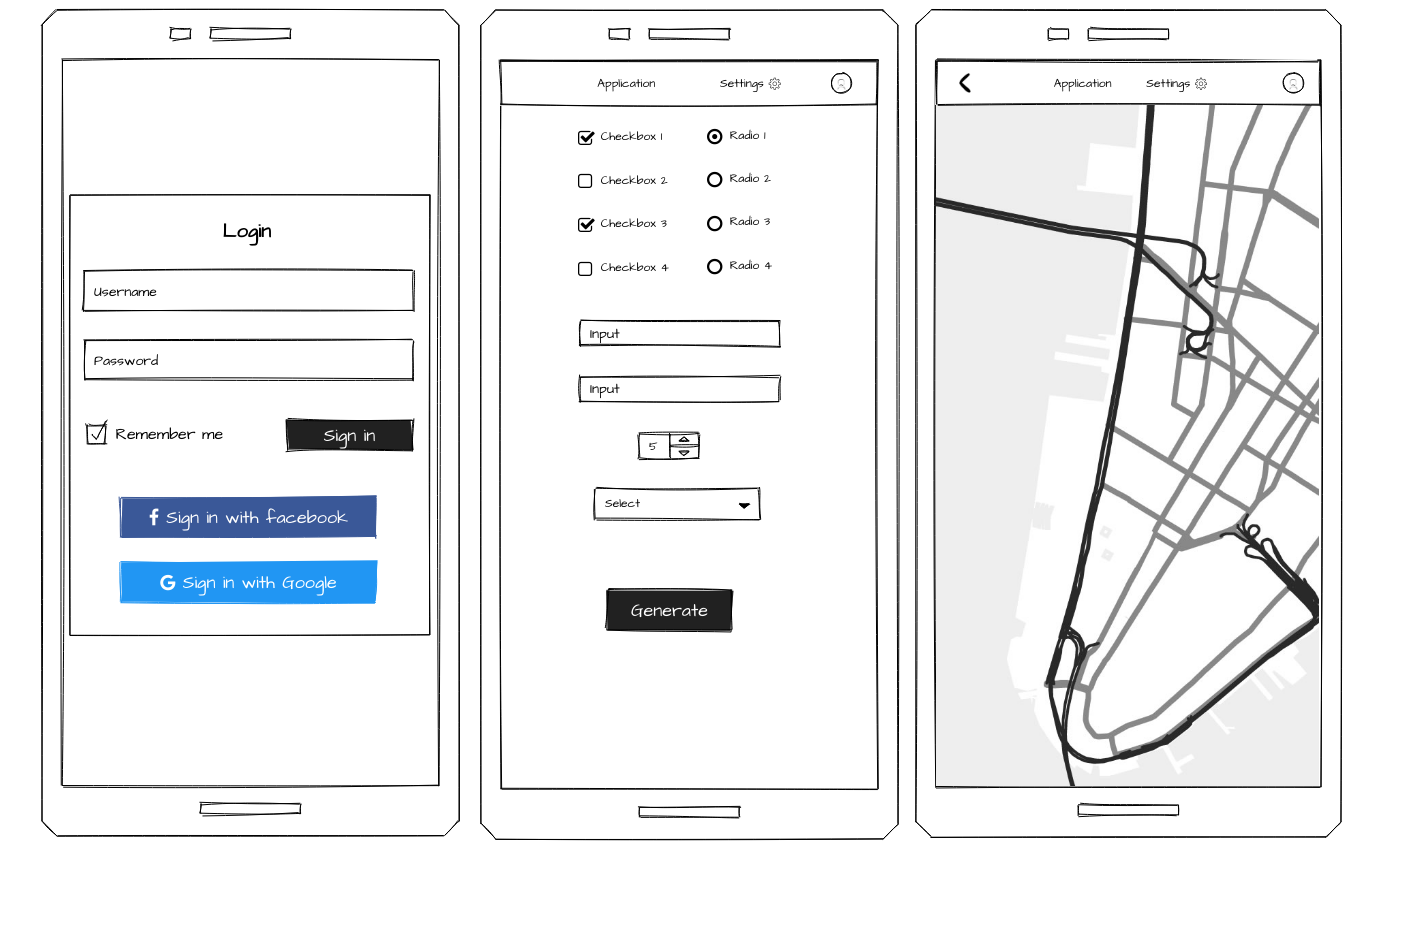
\includegraphics[width=\linewidth]{./graphics/wireframes.png}
    \caption{Wireframes.}
    \label{fig:wireframes}
\end{figure}

Figuur \ref{fig:wireframes} toont hoe de applicatie eruit zou kunnen zien. 
Dit is echter een eerste versie,
die nog verder uitgewerkt zal worden met behulp van de nodige analyse van huidige route-apps.
Het is de bedoeling dat een gebruiker/loopfanaat gemakkelijk een route kan genereren op basis van verschillende parameters. Deze route bevat dan ook een weersverwachting. 

\printbibliography[heading=bibintoc]

\end{document}